\documentclass[epsf]{article}
\usepackage{amsmath,amsthm,amsfonts,latexsym,amscd, framed}
\usepackage{graphicx}

\textwidth=6.0truein\hoffset=-.5truein
\textheight=8.5truein\voffset=-.5truein

\begin{document}
%\maketitle
\newcommand{\R}{\mathbb{R}}
\newcommand{\noi}{\noindent}
\newcommand{\bs}{\bigskip}

%%%%

\begin{center}
{\Large Project \#4: Phase Portraits for Linear DE Systems\\
\vskip 2mm
TA Guide pt 1}
\end{center}

\noi{\bf 1.} Have the students work in groups of 2 or 3 - and only hand out one worksheet per group.  It will be easier for them to look back and forth between the questions and the phase portraits if it's NOT printed two-sided; so this once, print the pre-work as two pages stapled together or hand the pages out separately.   Have them start with system (a) and give them a few minutes to narrow down which phase portrait(s) might be the right one.\\



\noi{\bf PW 1} Choose the phase portrait (on the next page) that corresponds to each the following DE systems.  As you are thinking about the problems, take notes on why you chose or ruled out a certain phase portrait.  You can use your notes from section to help you write justifications for your choices on the solutions page for DP\#4.

\begin{itemize}
\item[(a)] The system $\vec{\bf x}' = \begin{bmatrix}-1 & 1\cr\ \ 0 & 1 \end{bmatrix}\vec{\bf x}$ has general solution
$\vec{\bf x}(t) = c_1e^{-t}\begin{bmatrix}1 \cr0 \end{bmatrix} + c_2e^{t}\begin{bmatrix} 1 \cr 2 \end{bmatrix}$.

\noi{\bf 2.} We sketched a saddle in class on Tuesday, so this should be familiar to them.  After about 2 minutes or so, ask the class if they can rule out some choices or narrow it down.  Be stubborn and make them give you something to work with.  If a student suggests ruling some phase portraits out, ask them to explain why and write down those explanations on the board so everyone can follow.  Be neutral and ask the class if they agree or disagree with their peers' reasoning.  Some ideas that might come up:
\begin{itemize}
\item The ``eigen-solutions'' are real, so you should see two straight-line solution trajectories in the phase portrait.  This is still a bit confusing for many of them, so you may want to explain why this happens in some detail if a student brings it up.  This rules out A-C and I-L.
\item The eigenvalues have different signs, so one ``eigen-solution" moves towards the origin, while the other ``eigen-solution'' moves away from the origin.  This rules out D-F.
\item They can sketch the eigen-solutions (or identify them) to choose between G and H.
\end{itemize}

\item[(b)]  The system $\vec{\bf x}' = \begin{bmatrix}2 & 2\cr 1 & 3 \end{bmatrix}\vec{\bf x}$ has general solution
$\vec{\bf x}(t) = c_1e^{4t}\begin{bmatrix}1 \cr1 \end{bmatrix} + c_2e^{t}\begin{bmatrix} -2 \cr \ \ 1 \end{bmatrix}$.

\noi{\bf 3. } Repeat the same procedure for each of the other parts: give them a minute to narrow down the search, then ask the class to share what they came up with.  Write down their ideas and reasoning so the whole class can follow. 
\begin{itemize}
\item Again, we have real ``eigen-solutions'' so you'll see the straight-line solution trajectories in the phase portrait, ruling out A-C and I-L.
\item The eigenvalues are positive, so all solution trajectories move away from the origin.  This rules out F-H.
\item They may also look for the eigenvector directions in the phase portrait, which only leaves D and F as possibilities.
\item In the end, only D makes sense.  Note that we call this a \textit{nodal source}.
\end{itemize}

\item[(c)] The system $\vec{\bf x}' = \begin{bmatrix}0 & -2\cr 2 & \ \ 0 \end{bmatrix}\vec{\bf x}$ has general solution
$\vec{\bf x}(t) = c_1\begin{bmatrix}-\sin(2t) \cr \cos(2t) \end{bmatrix} + c_2\begin{bmatrix}\cos(2t)\cr \sin(2t) \end{bmatrix}$.

\begin{itemize}
\item Here we don't have any straigh-line solutions, so this rules out D-H.  Ask them what kind of eigenvalues this matrix must have (real? complex? purely imaginary?).
\item They can probably also tell that these trajectories are periodic or that they aren't shrinking or growing... This rules out I-L.
\item This part may be tough for them, but ask what kind of shape $\begin{bmatrix}\cos(2t)\cr \sin(2t) \end{bmatrix}$ traces out in the plane.  Give them a minute to think about it in their groups.  Once they get ``circle'', ask them what curve $\begin{bmatrix}-\sin(2t) \cr \cos(2t) \end{bmatrix}$ traces out.  This should narrow it down to choice B.
\item Ask them how they could tell (if the phase portraits weren't given) that the circle goes counter-clockwise?  They should be able to check by using the matrix of the system to find tangent vectors along the $x$- or $y$- axes.
\end{itemize}

\item[(d)] The system $\vec{\bf x}' = \begin{bmatrix}-1 & \ \ 1\cr -2 & -1 \end{bmatrix}\vec{\bf x}$ has general solution
$\vec{\bf x}(t) = c_1e^{-t}\begin{bmatrix}\sin(\sqrt{2}t) \cr\sqrt{2} \cos(\sqrt{2}t) \end{bmatrix} + c_2e^{-t}\begin{bmatrix}-\cos(\sqrt{2}t)\cr \sqrt{2}\sin(\sqrt{2}t) \end{bmatrix}$.

\begin{itemize}
\item  Here we don't have any straigh-line solutions, so this rules out D-H.  Ask them what kind of eigenvalues this matrix must have (real? complex? purely imaginary?).
\item  They will be able to tell that the trajectories are shrinking towards the origin because the exponent has a negative sign (you may want to note that this is the real part of the complex conjugate eigenvalues) -- which rules out A-C and J-K.  
\item To decide between I and L they will probably have to check the tangents of solution trajectories along the $x$-axis - give them a minute to do this and then come together and talk about the result.  You should be left with only choice I.
\end{itemize}

\end{itemize}

\newpage

Each of the following is a phase portrait for a $2\times 2$ linear DE system. \\


\begin{center}
A 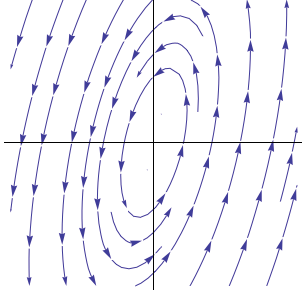
\includegraphics[width=40mm]{center1.png}\hspace{0.6 cm}B 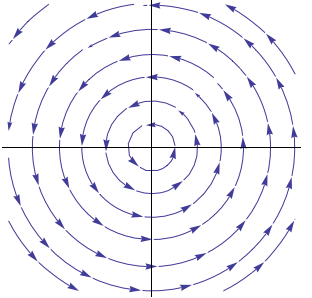
\includegraphics[width=40mm]{center2.png}\hspace{0.6cm}C 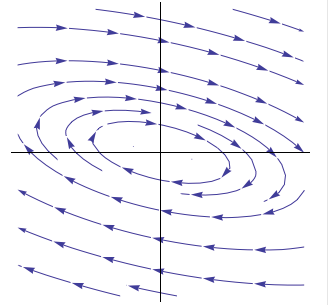
\includegraphics[width=40mm]{center3.png}\\

\vskip 1cm
D 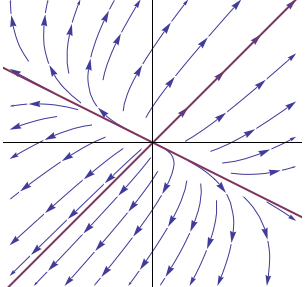
\includegraphics[width=40mm]{source1.png}\hspace{0.6 cm} E 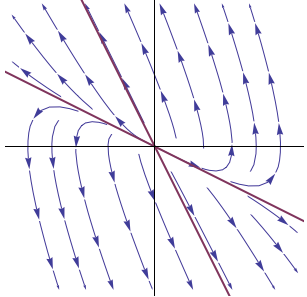
\includegraphics[width=40mm]{source2.png}\hspace{0.6 cm} F 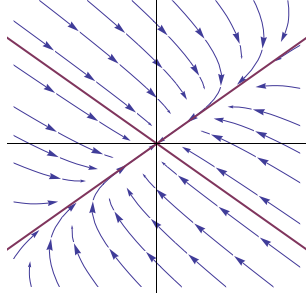
\includegraphics[width=40mm]{sink.png}\\
\vskip 1cm
G 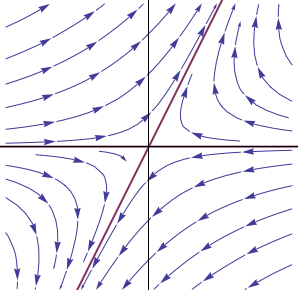
\includegraphics[width=40mm]{saddle.png}\hspace{0.6 cm} H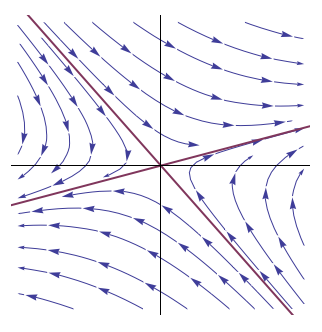
\includegraphics[width=40mm]{saddle2.png}\hspace{0.6 cm} I 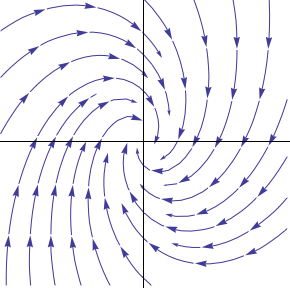
\includegraphics[width=40mm]{stable_spiral.png}\\
\vskip 1cm
J 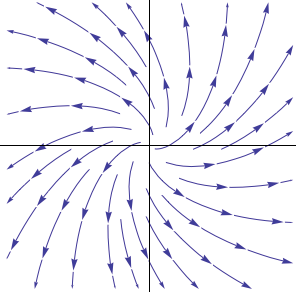
\includegraphics[width=40mm]{spiral_source.png}\hspace{0.6 cm} K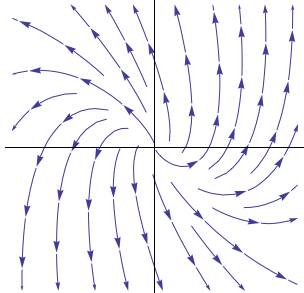
\includegraphics[width=40mm]{spiral_source2.png}\hspace{0.6 cm} L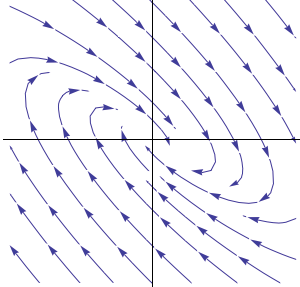
\includegraphics[width=40mm]{stable_spiral2.png}\\
\end{center}

\end{document}